% 
% Permission is granted to copy, distribute and/or modify this document
% under the terms of the GNU Free Documentation License, Version 1.2
% or any later version published by the Free Software Foundation;
% with no Invariant Sections, no Front-Cover Texts, and no Back-Cover
% Texts.  A copy of the license is included in the section entitled "GNU
% Free Documentation License".




%%%%%%%%%%%%%%%%%%%%%%%%%%%%%%%%%%%%%%%%%%%%%%%%%%%%%%%%%%%%%%%%%%%%%%%%%%%%%%%%%%%%%%%%%% 
\section{Developers Guide}

This section presents some information intended for the developer. It makes up the general specification design for the architecture of the OTADS module. the architecture is given in Figure~\ref{fig:architecture}.\par

\begin{figure}[htb]
    \begin{center}
        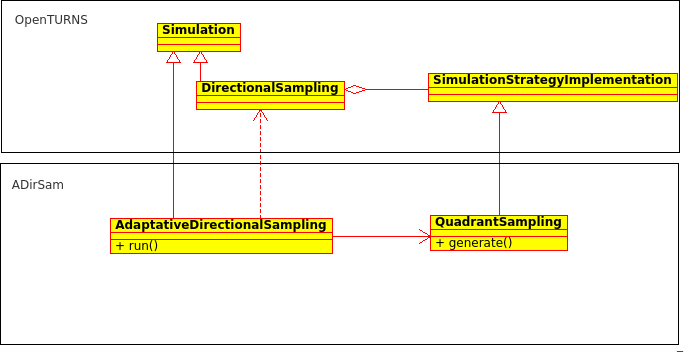
\includegraphics[scale=0.8]{architecture.png}
        \caption{OTADS classes.}\label{fig:architecture}
    \end{center}
    \label{fig:architecture}
    \caption{Architecture of the OTADS module.}
\end{figure}

\paragraph{AdaptiveDirectionalSampling}

The class AdaptiveDirectionalSampling derives from the Simulation class and implements the ADS-2 algorithm as well as its variants.\\

\paragraph{QuadrantSampling}

The class QuadrantSampling derives from SamplingStrategyImplementation. It enables the conditinal sampling of directions in a given quadrant.\\


